% !TEX root = ../thesis_main.tex



%%%% --- * --- %%%%	
\clearpage
\chapter*{Long Comments}
\addcontentsline{toc}{chapter}{Long Comments}

\note[gg, nolist]{From Gerald:
\\...\\
Hi Melissa,
\\...\\
Attached is the report by Georg. I contains many valid points, and even for those where I'm not fully on board, it's clear that this has to be addressed. To be clear: This is not really that big of a deal. The actual work is not questioned in any way, and that's of course the really relevant part in the end. But it does have to be framed within a context, especially for the non-experts. I should have probably called off things like the handwritten appendix earlier, but thought that the committee members would ask for that in passing (on the basis that everything in the thesis must stand on its own, which those personal notes arguably don't; if this is relevant, it should be typed up).
\\...\\
I will write to the other committee members and call off their effort on this version, because Georg already won't sign off on it, so there is not point for them to go through it, as they most likely will agree with his points.
\\...\\
The course of action will now be for you to address these issues and then we'll resubmit.
\\...\\
I'm not entirely sold myself on a full "Standard Model intro" in the sense that the beta decay work stands on its own, and can be told as its own story. This is reflected by the fact that JTW predates the SM is is still fully relevant. So I'd go a somewhat light SM exposure. The most important goal is to make the non-experts comfortable in introducing what this is all about.
\\...\\
This will also bolster the citation count, which indeed looks suspiciously low (even though i'm not keen on such bean counting arguments).
\\...\\
Gerald
}

%%%%%%%%%%%%%%%%%%%%%%%%%%%
\note[jbn, nolist]{John's suggestions for fixing the stuff that Georg wanted fixed -- that giant email.
\\...\\
hi Melissa,
\\
Gerald will soon send good clear corrections from a committee member. It will be clear you need to address those, and it will be clear what to do.
\\
Please read those first, and start answering them. Maybe then (and only then!) you will find two suggestions useful:
}
\note[jbn, nolist]{
i) Among the necessary technical corrections, there's a solid request for more background info. I think you know what to do.
\\...\\
A large thing is some kind of extra qualitative description of what the SM is. You could do that qualitatively without any trouble.
\\...\\
You might point out some part of this:
\begin{itemize}
	\item the charged weak interaction you're writing down predates the Weinberg-Salam model by more than a decade. The version you've written down assumes protons and neutrons are fundamental particles.
	\item The exchange boson is much heavier in mass than the energy and momentum in the decay, so it can be approximated by an interaction with zero range. 
	\begin{itemize}
		\item Fermi did that very early on, 
		\item and Gamow and Teller added a process that change the nucleon spin. 
		\item Lee and Yang, which you cite, added the possible currents with different Lorentz transformations (do you mention that since any further combination of Dirac matrices can be reduced to these, so they span the space), and the possibility of parity violation by writing out helicity projections for the leptons. I.e. Lee and Yang assumed some fields (the nucleons and leptons) and a general interaction preserving the symmetries of the theory, which by definition is then an effective field theory.
	\end{itemize}
	\item Feynman and Gell-Mann's 1958 paper is the one that postulated V-A, again a decade before Weinberg-Salam, and they did this by making analogies between the boson exchanged and the photon, i.e. an analogy between the charged weak interaction and the electromagnetic current, so you could cite them instead of saying "SM predicts everything"
\end{itemize}
People had assumed there was a massive boson exchanged for a very long time.
\\
What Weinberg (and, independently, Salam) did was come up with a consistent mathematical theory of massive bosons, incorporating Yang Mills gauge theory (looks like E\&M but with nonabelian operators) to do that, and the result was the weak neutral interaction prediction.
}
\note[jbn, nolist]{
ii) Similarly, answering how the results fit into the bigger picture is what you wanted to do.
\\...\\
I'm convinced that you don't want to do a full review of all beta decay experiments.
\\...\\
But you could say the Fierz term has been constrained by the energy spectrum and by the energy dependence of the beta
asymmetry, cite the best paper in the neutron and maybe the UCNA one as well, and use that figure I sent (I'm sending the improved version).
\\...\\
It is a good approximation to linearize the situation, i.e. this figure is good for small Cs and Ct. (A similar approach is being used in a letter coming out soon, and 3 referees did not nag them about it.)
}
\begin{figure}[htb]
	\centering
	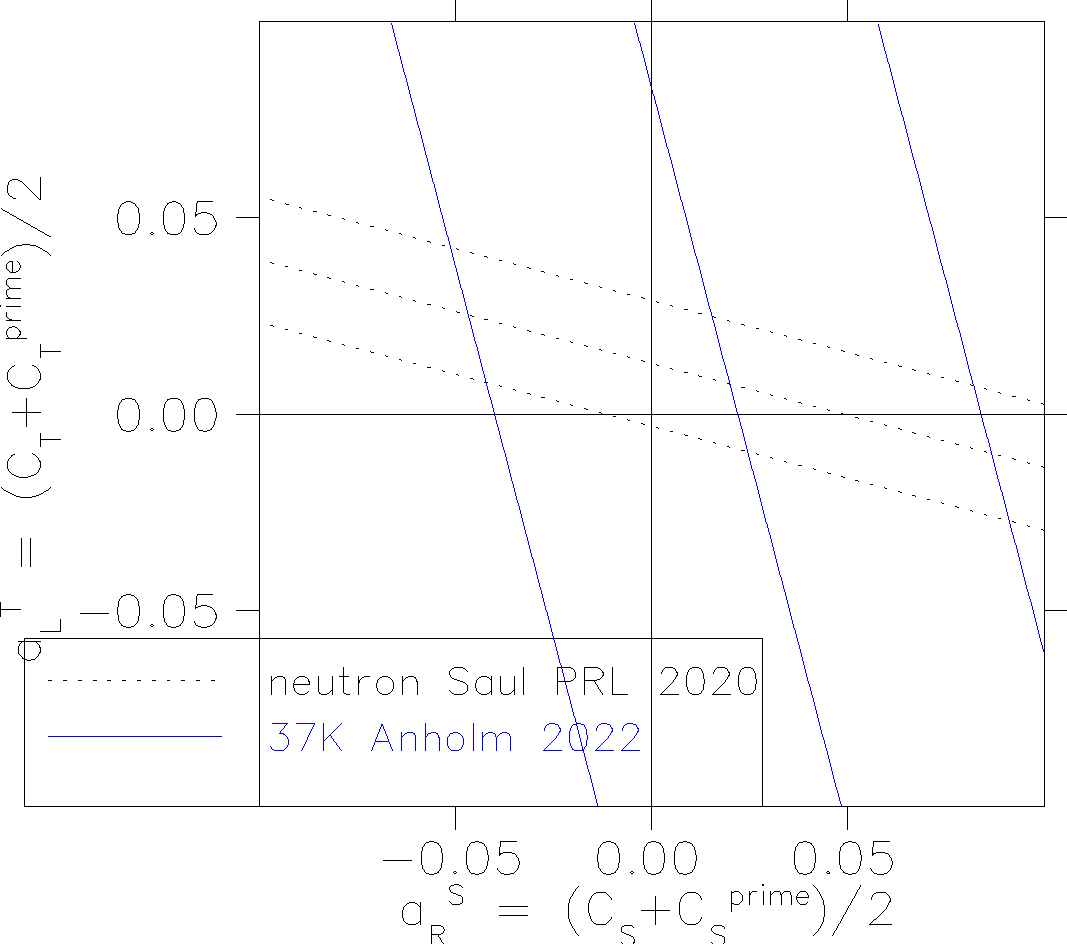
\includegraphics[width=.999\linewidth]{Figures/JB_exclusion.pdf}
	\caption[That exclusion plot from John.]{That exclusion plot from John.}	
	\label{fig:nuclearleveldiagram_new}
\end{figure}

\note[jbn, nolist]{Immediate follow-up email from John:  
\\...\\
another basic big point. What would it mean if there were nonzero Cs, Ct? 
\\
In the context of the more elegant SM, a theory of quarks and leptons and mathematically consistent interactions, that would imply the existence of at least one extra unknown exchange boson. The mass would not be measured, just its coupling
strenghts to the particles participating in the beta decay.
\\...\\
Maybe background to understand that includes:
\\
If one were to write the SM weak interaction, $C_A$ and $C_V$ and $C_A$ and $C_V g_A$ would all be constants with abs value 1.
The (1+- gamma\_5)'s are projection operators-- in the SM, the W boson only couples to left-handed nu's and right-handed antinu's
\\
('more will be said in the forward-looking Ch. 6.2 about tests of that part.)
\\
So all the known information about Ca and Cv is accounted for.
\\
($g_A = 1.26$ for the neutron... it's not equal to 1 because of strong interactions between the quarks in the neutron.)
}

%%%%%%%%%%%%%%%%%%%%%%%%%%%
\FloatBarrier
\note[gs, nolist]{From Georg Schreckenbach:
\\
Re: Melissa Anholm, Ph.D. thesis, version April 18, 2022
\\
In response to your request for pre-evaluation of Melissa Anholm’s Ph.D. thesis, dated April 18, 2022, I believe that the thesis in its current form is \emph{not} ready for distribution.
}
\note[gs, nolist]
{
In my view, the following are critical problems:
\begin{enumerate}
    \item 1. The thesis in its current form is completely missing any embedding into a “bigger picture”.
    This would be the task of the Introduction chapter primarily, but should also significantly permeate other parts such as, notably, the conclusions. One could phrase this in the form of questions, including – but certainly not limited to – the following:
    \begin{itemize}
        \item - What is the Standard Model?
        \item - Why are we even searching for “physics beyond the standard model”? Why is there a need or desire to do so?
        \item - What other efforts have been or are being made to search for physics beyond the standard model? Have any of them been successful? If so – or if not, what does this mean?
        \item - Closely related to the previous question, how does the current work fit into this overall effort? What is the unique contribution here?
	\end{itemize}
    Etc.
%%%\end{enumerate}
%%%...\\
%%%}
%%%\note[gs, nolist]{
%%%\\...\\
%%%\begin{enumerate}
%%%	\setcounter{enumi}{1}
    \item 2. These aspects should be picked up in the Conclusions. What do the results mean for the “big
    picture”? Again, how do the fit in with the other efforts, prior, concurrent, or planned? Etc.
\end{enumerate}
...\\
}
\note[gs, nolist]{
\\...\\
\begin{enumerate}    
	\setcounter{enumi}{2}
    \item 3. As an outsider, it is my understanding that the author worked as part of a larger collaboration.
    It would be beneficial to clearly lay out what her unique contributions are. This could be
    done, for instance, in the Introduction, and/or the Conclusions.
\end{enumerate}
}
\note[gs, nolist]{
\begin{enumerate}    
	\setcounter{enumi}{3}
    \item 4. Formulas and symbols contained in these need to be defined, as do symbols that appear in the
    text. Currently, this is only done partly. It starts right at the beginning with Eq.~\ref{eq:betaplus_decay} (formerly 1.1) and continues throughout. Sure, one can of course guess the meaning of the symbols in Eq.~\ref{eq:betaplus_decay} – but one should not have to guess! – and this is certainly not true for later equations. (For instance, I have no idea about the meaning of most of the symbols in Eq.~\ref{equation:integrated_jtw_INTRODUCTION} (formerly 1.9), to give but one example.)
\end{enumerate}
}
\note[gs, nolist]{
\begin{enumerate}    
	\setcounter{enumi}{4}
    \item 5. Similarly, several figures need better explanations, starting with Fig. 1.1. Which, btw., also needs a source attribution (unless it was created by the author) and, presumably, a copyright note. Similar comments apply to various other figures as well.
\end{enumerate}
}
\note[gs, nolist]{
\begin{enumerate}    
	\setcounter{enumi}{5}
    \item 6. At first glance, I find a bibliography that contains only 28 entries to be problematic for a Ph.D. thesis. This goes, to some degree, back to my earlier points about embedding the work in the “bigger picture” – doing so would necessarily lead to several additional references – but it might be more than that.
\end{enumerate}
}
\note[done, nolist]{
\begin{enumerate}    
	\setcounter{enumi}{6}
    \item 7. Appendix C, adding scanned pictures of handwritten notes as figures that, moreover, seem not to be referenced at all, is – well – problematic. I don’t think that it conforms to the instructions as per Supplemental Regulations either (though I did not explicitly check).
\end{enumerate}
}

\note[gs, nolist]{
\\...\\
Given these various issues, I have not fully read the thesis in detail; I have instead focused on the question at hand: what is needed for the thesis to be in a form that can be distributed? I will provide a more formal report on the version of the thesis that I will receive from FGS.
}
\note[gs, nolist]{
Besides, there are some additional points that I would suggest for modification but that do not, in my mind, prevent distribution. These include:

\begin{enumerate}    
	\setcounter{enumi}{7}
    \item 8. The abstract in its current form comprises 186 words or so. The FGS regulations allow for
    350 words maximum; I would encourage the author to make better use of that space – not the
    least in light of my earlier comments regarding the “big picture” and such.
    \item 9. The thesis would benefit from a list of abbreviations.
    \item 10. P. 93 contains a reference to “Figure ??”
    \item 11. Likewise, p. 98, a reference to “Ch. ??”, as well as a reference to “our recent PRL article” –
    the latter needs to be referenced properly!
    \item 12. I have no idea what the title of Appendix B means. It is for sure original and even funny
    though ... Also, the actual appendix title in the thesis is not the same as that listed in the TOC.
\end{enumerate}
}


\begin{figure}[htb]
	\centering
	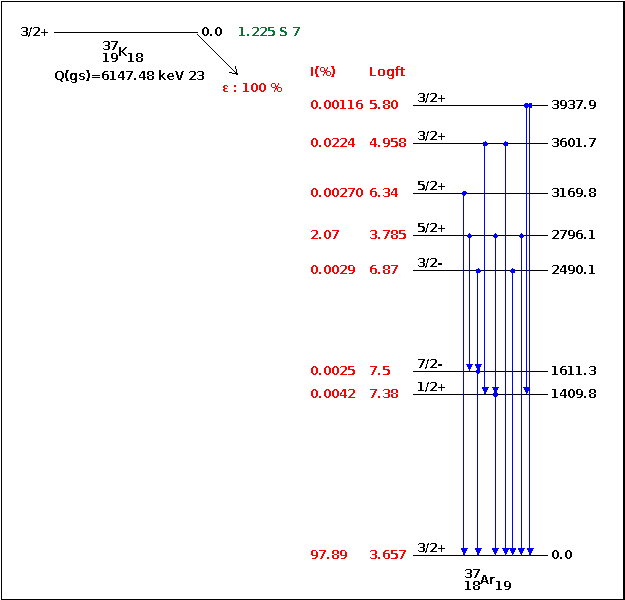
\includegraphics[width=.999\linewidth]{Figures/decayscheme_nndc.png}
	\note[orange, nolist]{Authors: John Cameron, Jun Chen and Balraj Singh, Ninel Nica.
	\\
	Citation:Nuclear Data Sheets 113, 365 (2012)
	\\...\\
	Also, it's generated by the page from:  National Nuclear Data Center (NNDC) at Brookhaven National Laboratory.  Possibly from the NuDat3 database.
%	\\
%	https://www.nndc.bnl.gov/nudat3/decaysearchdirect.jsp?nuc=37K&unc=NDS
	}
	\caption[New 37K decay scheme]{A newer, better, less generated-by-Dan level diagram for the decay of $\isotope[37]{K}$.}	
	\label{fig:nuclearleveldiagram_new}
\end{figure}


%%%%%%%%%%%%%%%%%%%%%%%%%%%
\FloatBarrier

\note[jbn, nolist]{Suggestions from John on listing my contributions that need to be mentioned and/or general stuff that needs to be mentioned:
\\
Georg wants you to list your contributions in the intro, good.
\\...\\
First, in Section 2.4 the sentence after Harvey and Murray are referenced could be "There are some details of the present implementation of the AC MOT in Ref.~\cite{thesis}, done with a separate MOT geometry from
this beta decay work."
\\
(Presently your thesis is Ref. 14, which is only cited so far for Fig. 2.1)
\\...\\
*you need a subsection in Section 2.4 "The AC-MOT and Polarization" on your field trimming.
\\...\\
Time-constant ambient fields were trimmed in all dimensions using two horizontal pairs of Helmholtz coils and the AC MOT coils for the vertical direction.
These ambient B fields were first trimmed to be near zero using a giant magnetoresistance 3-axis probe at the trap center, with the MCP assembly removed and the vacuum chamber up to air.
\\...\\
Final trimming was done by optimizing polarization of stable $^{41}$K atoms with the apparatus assembled (cite[Fenker PRL Suppl Mat] has some details).
\\...\\
The AC MOT and polarization B fields were generated by SRS DS345 arbitrary waveform generators, amplified by
Matsusada bipolar 20 KHz bandwidth 80A 20V amplifiers. The waveforms were carefully trimmed in amplitude and time to minimize B fields from eddy currents during the optical pumping cycle, again with the MCP assembly removed and the vacuum chamber up to air.
\\...\\
The bipolar amplifier bandwidth was inadequate when using current control mode, so voltage control had to be used, a much more time-exacting process requiring empirical iteration. These waveforms are not the same for the top and bottom coils, as during the optical pumping cycle one coil had to be flipped with respect to the MOT cycle to create the uniform vertical field for optical pumping by a Helmholtz rather than antiHelmholtz configuration.
\\
The beta detector full assemblies were in place during the field trimming.
\\...\\
All materials near the trap cloud are chosen to minimize both magnetic permeability to suppress time-constant B field gradients and conductivity to suppress eddy currents. E.g., the E field electrodes are made from either glassy carbon semiconductor or titanium alloy. A copper ring (not pictured in Fig. 2.5) with a slit mounted on each beta detector stainless steel reentrant flange suppresses the worst eddy currents fighting the B field along the z-axis. These designs were all confirmed by finite element calculations of another collaboration member.
}


\note[jbn, nolist]{
I think you've neglected where the fT value and prediction for Abeta come from, entirely, and still don't have an equation for b\_Fierz in terms of Cs and Ct.
\\...\\
You had a note to do this, and in desperation I encouraged you to leave it out.
I was wrong and Georg is right-- the whole SM prediction for Abeta makes no sense this way, and something about it needs to be there.
\\...\\
there are two ways to add a dedicated section in ch 1:
\begin{itemize}
	\item i) by writing the equation for the rate in terms of Vud and rho (the G-T matrix element over Fermi squared), and saying Shidling et al. gets rho from that by assuming Vud from the 0+ to 0+ decays. (You had a note "Do the master equation!" which I think I said you needed to leave out, but I was probably wrong.) But then you have to define all the small corrections, which is a lot of physics.
	\item ii) Write the SM equation for Abeta in terms of rho, to give you the SM prediction for Abeta. State that recoil order corrections are in Appendix X. (If that's now a collaboration note? cite that there are recoil corrections considered in Appendix X-1 and a collaboration note).
	\item iii) Such a section would then naturally end with b\_Fierz in terms of Cs and Ct, a natural followup to what you've written.
	\\
"JTW does the Dirac matrix traces necessary to write down the decay rates in term of the Lee-Yang Lagrangian's parameters.
The prediction for b\_Fierz is " " which is zero in the SM." \textbf{even with recoil-order corrections} (there is no recoil order correction with the same m/Ebeta dependence).
\\
Then and only then will the final addition of the bFierz plot will make sense.
\end{itemize}
%
OR, more likely:
\\
\textbf{leave out i)}.
\\
Say in text that Shidling et al. (I've added the reference in a sticky note for the figure) hands you rho (the $M_{GT}/M_F$ ratio prediction) using as input the absolute rate, Vud from the 0+ to 0+ beta decays, and calculations of isospin mixing and radiative corrections (cite[shidling]) for details beyond the scope of this thesis. The sign of rho comes both from a shell model by Ian and by if it were flipped Abeta would be off by an enormous factor. 
\\...\\
Then you would just need \textbf{ii and iii}.
}
\note[jbn, nolist]{
As a reward for reading this far, I'll admit I wrote the bFierz m/E dependence wrong in the sticky notes in ch 1, sorry.
}

%%%
\note[jbn, nolist]{first, actually, Ben writes a good summary of Ft mirror equation in terms of Ft0+ to 0+ in the PRL, you could just use that in Ch. 1 and it would help enormously. (Of course now I'm scared because it doesn't mention isospin mixing is different for 37K and the others, and that should be in the numerator as (Ft0to0/Ft37K) well as in rho, shouldn't it? I would need to compare to Shidling's expressions to sort this out.)
}
\note[jbn, nolist]{
I said Ft wrong. I think you must know what to do.  
\\
F is the lepton phase space integral.
\\
(Decay rate)/F is then a dimensionless quantity proportional to |matrix element|$^2$, which you could call the intrinsic strength of the transition.
\\
People instead consider the inverse quantity denoted Ft defined as F*t\_1/2, so if log\_10(Ft) is smaller, the strength is larger.
\\...\\
So e.g. t\_1/2 is wildly different for the 0+ to 0+ decays (t1/2 for $^{14}$O is a minute, not a second like 38mK) but once you correct for the wildly different phase space (the Coulomb energies and therefore the decay Q-value smoothly grow, and phase space goes like $Q^5$) the Ft rates are close (closer once percent corrections from isospin mixing and nucleus-dependent radiative corrections are applied).
}
\note[jbn, nolist]{
...
\\
(That equation is fine-- I was confused earlier.) You can mention that script{Ft} has isospin-breaking and other theory corrections beyond the scope of the thesis, and cite Shidling for those. This equation, along with the Abeta equation in terms of rho (you should not include the right-handed currents in Ben's Abeta equation and re-state that your thesis is working on scalar and tensor in your title) then sets up the inputs you need for the Abeta prediction.
}
%%%

\note[jbn, nolist]{Chapter 2 corrections from John:
\\
all of these are trivial except the last, which counts as a glaring omission.
\\
\begin{itemize}
	\item *section 2.1.3 "using a Helmoltz coil" add "but with currents in opposite direction." (saying it correctly here then implicitly defines anti-Helmholtz which you use correctly later for the AC MOT)
	\item *It would be simplest to write down what you mean by a quadrupole field. You could say: "approximately in our geometry near the trap center
	\\
	$\vec{B} = 2 B_o z \hat{z} - (B_0 x \hat{x} + B_0 y \hat{y})$
	\item *section 2.4 near end "divergencelessness" is not a word. It's obvious how to fix it ''since del dot B =0 in a current-free region..."
	\item 2.5.1 "roughly" -> "approximately" The Efield is not rough at all, it's pretty good really. 
	\\
	Is the rMCP really just a 2-plate chevron in 2014? I don't remember. Why can't I find Ben's thesis?
	\item *2.5.1 state clearly in an extra paragraph at the end that the polarization-determining data was taken with the rMCP, while the Abeta and bFierz data were taken with the eMCP. The polarization was assumed to be the same during the Abeta+bFierz data. This is backed up by constant 41K polarization data for weeks
of optimization, with all optical pumping and B field switching parameters kept constant. Ambient magnetic field changes of 50 milliGauss could cause some polarization perturbations at the precision achieved, yet the stray fields are under control at that level. The TRINAT lab is in a basement well-shielded from the experimental hall by concrete with rebar, and though 50 mG fields are seen in that Hall from an open Helmholtz ion trap, they and the 5-ton crane produce negligible fields when measured at the atom trap. The cyclotron field makes 0.5 Gauss, predominantly vertical, and a smaller horizontal component, but trim Helmholtz coils at TRINAT are adjusted during calibrations with cyclotron on vs. off, and of course the cyclotron is on with constant field during the 37K delivery.
	\item *\textbf{You don't state the polarization achieved 99.1$\pm$0.1 percent anywhere that I can see., citing the publication.} You might also state that's important for Abeta but has much more precision than needed for the near-zero bFierz term.
	\\...\\
	You mention the polarization is different by approximately 0.3\% in Section 6.1 from the cut, but never say what P is.
	\\...\\
	Appendix A has ?? for a discussion of the changes of the polarization cut, so you need to clean up that \ref{}. It is presently in Section 6.1.
\end{itemize}
}











%%%% --- * --- %%%%	
%%%%%%%%%%%%%%%%%%%
%\FloatBarrier
\clearpage

\note[white, nolist]{Old Notes!} \noindent

\note[jb1, nolist]{JB on intuitive concepts that are missing (are they *still* missing?!?):  
\\
The SM couples to left-handed neutrinos and right-handed antineutrinos. Since the neutrinos only have weak interactions, there are no right-handed nu's nor left-handed antinu's in nature. The neutrino asymmetry $B_\nu$ is a number with no energy dependence. 
\\
Similarly, the SM weak interaction only couples to right-handed positrons and left-handed electrons. Since these are massive particles, the average helicity of positrons is not 1, but instead v/c. One can always boost to a frame where the positron keeps its circulation but is moving in the opposite direction. This is why the beta asymmetry is A v/c, not just A.
\\
The Fierz term's additional energy dependence of m/E also comes from helicity arguments, stemming from the fact that it still is coupling to SM nu's and antinu's only, so the beta's are generated with wrong handedness.  
\\
The details are built at 4th-year undergrad level in Garcia's paper with his student and postdoc~\cite{hong_sternberg_garcia}.
}
%\note[jb1]{JB on intuitive concepts that are missing:  
%\\
%The beta asymmetry dependence on the Fierz term only comes through the normalization of $W(\theta) = 1 + \bFierz m/E + \Abeta \cos(\theta)$.
%\\ i.e.:
%\\$W'(\theta) = 1 + \Abeta/(1+ \bFierz m/E) \cos(\theta)$.  (the angular distribution must be unity where cos(theta) vanishes, by definition).
%}

.
\note[org, nolist]{I have legit just deleted a section in Ch.6:  "Relation to Other Measurements and New Overall Limits".  It's gone now.  Because it was stupid.  Only John's comments about what it might do in the future remain.}
\note[jb1, nolist]{JB on Ch.~\ref{sec:relation_to_other_measurements}:  "Relation to Other Measurements and New Overall Limits"
\\
6.3 might be better left to a collaboration memo. You have to decide what to do here,
and decide it quickly.
\\...\\
I already gave you the latest Perkeo Fierz paper,
and the info that we are relatively less sensitive to tensor by
by the ratio of Mgt$^2$ = 3/0.6 = 5.
\\...\\
so if you make a linearized exclusion plot of tensor vs. scalar as straight
lines with the uncertainty of bFierz, using Perkeo and your result, you
will see even with 0.09 uncertainty you compete with them on the scalar limit.
\\...\\
(However, see attached figure from my article with Alexandre on 38mK's
beta-nu scalar limit. I think the constraints on Lorentz scalars are hard to
compete with.)
}
\note[jb1, nolist]{JB says:   To put your work in context, please add at the end of that minimal S,T section, or at the end of "Our Decay" section
\\ ... \\
The best existing measurement of $\bFierz$ is in the decay of the neutron~\cite{Saul2020},
$\bFierz$ = 0.017 $\pm$ 0.021, consistent with the Standard Model prediction of zero.
Our measurement is strongly related, yet complementary.
In terms on non-Standard Model Lorentz current structures, to lowest order in the non-SM  currents the same equation applies:
\\
$\bFierz$ = $\pm$ $(C_S +C_S' + (C_T - C_T') \lambda^2)/( 1 + \lambda^2)$
\\
(the plus is for $\beta^-$ decay and the - for $\beta^+$ decay)~\cite{jtw}.  [to be continued...] }
\note[jb1, nolist]{[...continued from prev.]
\\
In our $^{37}$K case, $\lambda^2$ = $|M_{\rm GT}|^2$/$|M_{\rm F}|^2$ is close to 3/5 (the expected value j/(j+1) for a single j=3/2 d3/2 nucleon)~\cite{deShalit1963},
while for the neutron $\lambda^2$ is close to 3 (the expected value for an (j+1)/j j=1/2 s1/2 nucleon).
$|M_F|$, the Fermi matrix element, is nearly the same for both of these isospin = 1/2 decays (the largest correction is the larger isospin mixing of $\sim$0.01 in $^{37}$K).
So our observable is relatively less sensitive to Lorentz tensor currents, and will predominantly constrain or discover Lorentz scalar currents.
\\...\\ 
Full considerations would require a weighted fit of $\bFierz$ experiments and similar observables~\cite{Falkowski2021}, and are beyond the scope of this thesis.
The info from this thesis, values of $\Abeta$ and $\bFierz$ with their uncertainties, can together with the known $fT$ value (lifetime and
branching ratio) allow the community and/or the collaboration to include the results in a future constraint or discovery of scalar and tensor Lorentz currents
contributing to $\beta$ decay.}
\note[org, nolist]{End of John's comments on the section I deleted.}


%
%%%% --- * --- %%%%	
%
\clearpage

